% Options for packages loaded elsewhere
\PassOptionsToPackage{unicode}{hyperref}
\PassOptionsToPackage{hyphens}{url}
%
\documentclass[
  ignorenonframetext,
]{beamer}
\usepackage{pgfpages}
\setbeamertemplate{caption}[numbered]
\setbeamertemplate{caption label separator}{: }
\setbeamercolor{caption name}{fg=normal text.fg}
\beamertemplatenavigationsymbolsempty
% Prevent slide breaks in the middle of a paragraph
\widowpenalties 1 10000
\raggedbottom
\setbeamertemplate{part page}{
  \centering
  \begin{beamercolorbox}[sep=16pt,center]{part title}
    \usebeamerfont{part title}\insertpart\par
  \end{beamercolorbox}
}
\setbeamertemplate{section page}{
  \centering
  \begin{beamercolorbox}[sep=12pt,center]{part title}
    \usebeamerfont{section title}\insertsection\par
  \end{beamercolorbox}
}
\setbeamertemplate{subsection page}{
  \centering
  \begin{beamercolorbox}[sep=8pt,center]{part title}
    \usebeamerfont{subsection title}\insertsubsection\par
  \end{beamercolorbox}
}
\AtBeginPart{
  \frame{\partpage}
}
\AtBeginSection{
  \ifbibliography
  \else
    \frame{\sectionpage}
  \fi
}
\AtBeginSubsection{
  \frame{\subsectionpage}
}

\usepackage{amsmath,amssymb}
\usepackage{lmodern}
\usepackage{iftex}
\ifPDFTeX
  \usepackage[T1]{fontenc}
  \usepackage[utf8]{inputenc}
  \usepackage{textcomp} % provide euro and other symbols
\else % if luatex or xetex
  \usepackage{unicode-math}
  \defaultfontfeatures{Scale=MatchLowercase}
  \defaultfontfeatures[\rmfamily]{Ligatures=TeX,Scale=1}
\fi
% Use upquote if available, for straight quotes in verbatim environments
\IfFileExists{upquote.sty}{\usepackage{upquote}}{}
\IfFileExists{microtype.sty}{% use microtype if available
  \usepackage[]{microtype}
  \UseMicrotypeSet[protrusion]{basicmath} % disable protrusion for tt fonts
}{}
\makeatletter
\@ifundefined{KOMAClassName}{% if non-KOMA class
  \IfFileExists{parskip.sty}{%
    \usepackage{parskip}
  }{% else
    \setlength{\parindent}{0pt}
    \setlength{\parskip}{6pt plus 2pt minus 1pt}}
}{% if KOMA class
  \KOMAoptions{parskip=half}}
\makeatother
\usepackage{xcolor}
\newif\ifbibliography
\setlength{\emergencystretch}{3em} % prevent overfull lines
\setcounter{secnumdepth}{-\maxdimen} % remove section numbering


\providecommand{\tightlist}{%
  \setlength{\itemsep}{0pt}\setlength{\parskip}{0pt}}\usepackage{longtable,booktabs,array}
\usepackage{calc} % for calculating minipage widths
\usepackage{caption}
% Make caption package work with longtable
\makeatletter
\def\fnum@table{\tablename~\thetable}
\makeatother
\usepackage{graphicx}
\makeatletter
\def\maxwidth{\ifdim\Gin@nat@width>\linewidth\linewidth\else\Gin@nat@width\fi}
\def\maxheight{\ifdim\Gin@nat@height>\textheight\textheight\else\Gin@nat@height\fi}
\makeatother
% Scale images if necessary, so that they will not overflow the page
% margins by default, and it is still possible to overwrite the defaults
% using explicit options in \includegraphics[width, height, ...]{}
\setkeys{Gin}{width=\maxwidth,height=\maxheight,keepaspectratio}
% Set default figure placement to htbp
\makeatletter
\def\fps@figure{htbp}
\makeatother

\makeatletter
\makeatother
\makeatletter
\makeatother
\makeatletter
\@ifpackageloaded{caption}{}{\usepackage{caption}}
\AtBeginDocument{%
\ifdefined\contentsname
  \renewcommand*\contentsname{Table of contents}
\else
  \newcommand\contentsname{Table of contents}
\fi
\ifdefined\listfigurename
  \renewcommand*\listfigurename{List of Figures}
\else
  \newcommand\listfigurename{List of Figures}
\fi
\ifdefined\listtablename
  \renewcommand*\listtablename{List of Tables}
\else
  \newcommand\listtablename{List of Tables}
\fi
\ifdefined\figurename
  \renewcommand*\figurename{Figure}
\else
  \newcommand\figurename{Figure}
\fi
\ifdefined\tablename
  \renewcommand*\tablename{Table}
\else
  \newcommand\tablename{Table}
\fi
}
\@ifpackageloaded{float}{}{\usepackage{float}}
\floatstyle{ruled}
\@ifundefined{c@chapter}{\newfloat{codelisting}{h}{lop}}{\newfloat{codelisting}{h}{lop}[chapter]}
\floatname{codelisting}{Listing}
\newcommand*\listoflistings{\listof{codelisting}{List of Listings}}
\makeatother
\makeatletter
\@ifpackageloaded{caption}{}{\usepackage{caption}}
\@ifpackageloaded{subcaption}{}{\usepackage{subcaption}}
\makeatother
\makeatletter
\@ifpackageloaded{tcolorbox}{}{\usepackage[many]{tcolorbox}}
\makeatother
\makeatletter
\@ifundefined{shadecolor}{\definecolor{shadecolor}{rgb}{.97, .97, .97}}
\makeatother
\makeatletter
\makeatother
\ifLuaTeX
  \usepackage{selnolig}  % disable illegal ligatures
\fi
\IfFileExists{bookmark.sty}{\usepackage{bookmark}}{\usepackage{hyperref}}
\IfFileExists{xurl.sty}{\usepackage{xurl}}{} % add URL line breaks if available
\urlstyle{same} % disable monospaced font for URLs
\hypersetup{
  pdftitle={Gastcollege Communities that Care},
  pdfauthor={Harrie Jonkman},
  hidelinks,
  pdfcreator={LaTeX via pandoc}}

\title{Gastcollege Communities that Care}
\subtitle{NHLStenden HBO Integrale Veiligheidskunde}
\author{Harrie Jonkman}
\date{10/1/23}

\begin{document}
\frame{\titlepage}
\ifdefined\Shaded\renewenvironment{Shaded}{\begin{tcolorbox}[boxrule=0pt, breakable, borderline west={3pt}{0pt}{shadecolor}, interior hidden, enhanced, frame hidden, sharp corners]}{\end{tcolorbox}}\fi

\begin{frame}{Introductie}
\protect\hypertarget{introductie}{}
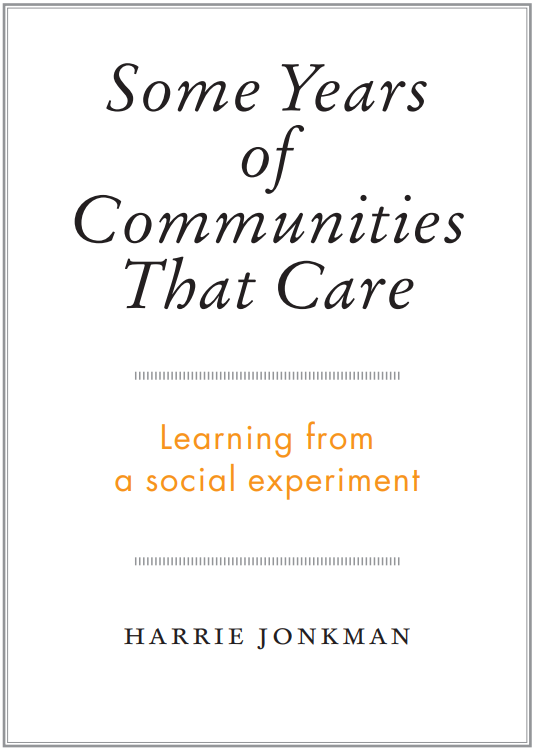
\includegraphics[width=2.08333in,height=\textheight]{images/CtC_voorkant.png}
\end{frame}

\begin{frame}{Opzet}
\protect\hypertarget{opzet}{}
\begin{enumerate}
\tightlist
\item
  Achtergronden en probleem
\item
  Uitgangspunten
\item
  De strategie
\item
  Vier kernelemementen
\item
  CtC-Nederland experiment (1999-2004)
\item
  CtC-Nederland interesse (2005-2015)
\item
  CtC-onderzoek (2008-2013)
\item
  CtC-Nederland recente ontwikkelingen (na 2015)
\item
  Andere landen
\item
  Discussie
\end{enumerate}
\end{frame}

\begin{frame}{1. Achtergronden en probleem}
\protect\hypertarget{achtergronden-en-probleem}{}
\end{frame}

\begin{frame}{MEG-problemen onder jonge mensen}
\protect\hypertarget{meg-problemen-onder-jonge-mensen}{}
\begin{itemize}
\tightlist
\item
  Mentale, emotionele en gedragsproblemen van adolescenten kunnen tot
  levenslange problemen en stoornissen leiden
\item
  Als samenleving hebben we verantwoordelijkheid jongeren gezond en
  veilig te laten opgroeien
\item
  In preventief opzicht kan er in jonge fase veel worden gedaan
\end{itemize}
\end{frame}

\begin{frame}{Fase van adolecentie}
\protect\hypertarget{fase-van-adolecentie}{}
\begin{itemize}
\item
  Fase van mogelijkheden
\item
  Fase van risico's
\end{itemize}
\end{frame}

\begin{frame}{MEG-problematiek jongeren}
\protect\hypertarget{meg-problematiek-jongeren}{}
\begin{itemize}
\tightlist
\item
  Delinquentie en geweld\\
\item
  Problematisch alcohol- en drugsgebruik\\
\item
  Schooluitval\\
\item
  Tienerzwangerschappen\\
\item
  Depressies en angsten
\end{itemize}
\end{frame}

\begin{frame}{Problematiek in Nederland}
\protect\hypertarget{problematiek-in-nederland}{}
\begin{figure}

{\centering 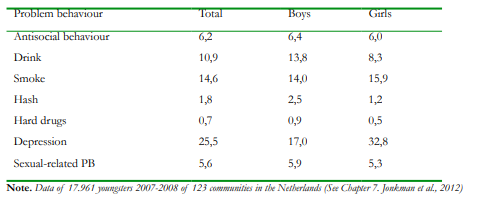
\includegraphics{images/TabelPG.png}

}

\caption{Prevalentie PG in Nederland}

\end{figure}
\end{frame}

\begin{frame}{2. Uitgangspunten}
\protect\hypertarget{uitgangspunten}{}
\end{frame}

\begin{frame}{Communities that Care}
\protect\hypertarget{communities-that-care}{}
\begin{itemize}
\tightlist
\item
  Een preventief interventiesysteem dat de gezonde en veilige
  ontwikkeling van jongeren in gemeenschappen (steden, wijken) wil
  bevorderen
\item
  Ontwikkeld vanaf eindjaren '80 door David Hawkins en Rico Catalano van
  de Social Development Research Group in Seattle (USA)
\item
  Bouwt voort op ontwikkelingen in de preventiewetenschappen
\end{itemize}
\end{frame}

\begin{frame}{Preventiewetenschappen}
\protect\hypertarget{preventiewetenschappen}{}
\begin{itemize}
\tightlist
\item
  Weinig inzichten in oorzaken van problemen
\item
  Geen programma's om dit aan te pakken
\item
  Weinig relatie tussen wetenschap, beleid en praktijk
\end{itemize}
\end{frame}

\begin{frame}{De theorie}
\protect\hypertarget{de-theorie}{}
\begin{itemize}
\tightlist
\item
  Ontwikkeling
\item
  Contexten
\item
  Sociale determinanten
\item
  Verschillende niveaus
\end{itemize}
\end{frame}

\begin{frame}{Ontwikkeling}
\protect\hypertarget{ontwikkeling}{}
\begin{itemize}
\tightlist
\item
  MEG-problematiek ontwikkelt zich zelden spontaan\\
\item
  Ontwikkelingspatronen waarin genen, ervaringen en omstandigheden op
  elkaar inwerken
\item
  Vroege ontwikkeling beïnvloedt cognitieve, sociale en mentale
  problemen van jongeren
\item
  Een groot deel van de problemen op volwassenleeftijd kennen oorsprong
  op jongere leeftijd
\end{itemize}
\end{frame}

\begin{frame}{Contexten}
\protect\hypertarget{contexten}{}
Overall speelt de ontwikkeling van jongeren zich in vier contexten af:

\begin{itemize}
\tightlist
\item
  Gezin\\
\item
  School\\
\item
  Vriendengroep\\
\item
  Wijk/stad/gemeenschap
\end{itemize}
\end{frame}

\begin{frame}{Sociale determinanten}
\protect\hypertarget{sociale-determinanten}{}
\begin{figure}

{\centering 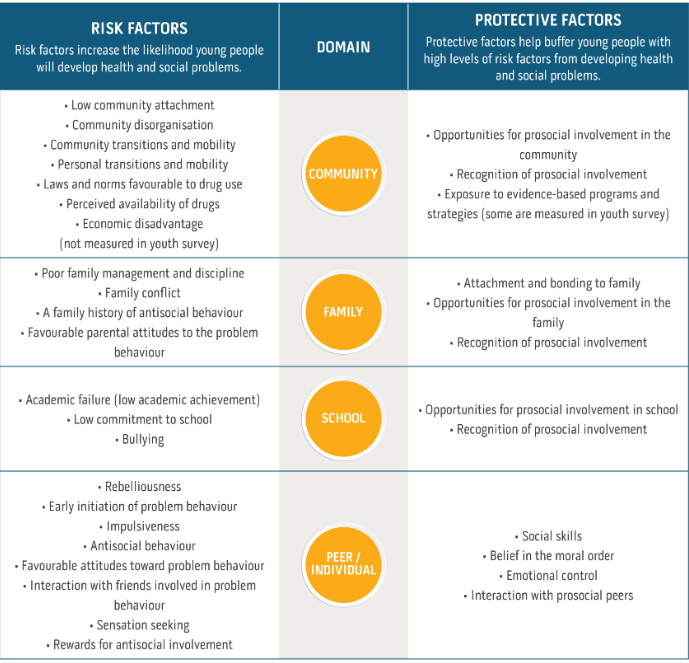
\includegraphics[width=2.08333in,height=\textheight]{images/Determinanten.png}

}

\caption{Risico en protectieve factoren}

\end{figure}
\end{frame}

\begin{frame}{Sociale determinanten risico's}
\protect\hypertarget{sociale-determinanten-risicos}{}
\begin{figure}

{\centering 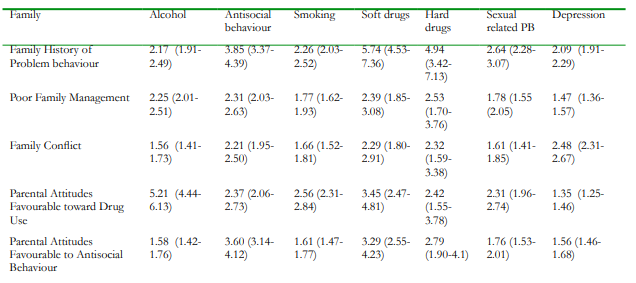
\includegraphics{images/RFFamilie.png}

}

\caption{Risico's in de familie}

\end{figure}
\end{frame}

\begin{frame}{Sociale determinanten protectie}
\protect\hypertarget{sociale-determinanten-protectie}{}
\begin{figure}

{\centering 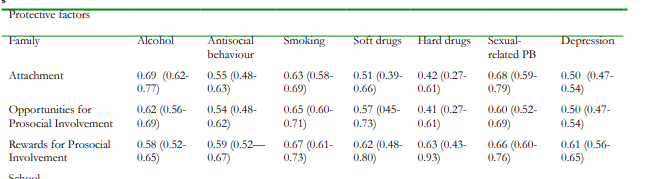
\includegraphics{images/PFFamilie.png}

}

\caption{Protectie in de familie}

\end{figure}
\end{frame}

\begin{frame}{Verschillende niveau's}
\protect\hypertarget{verschillende-niveaus}{}
\begin{figure}

{\centering 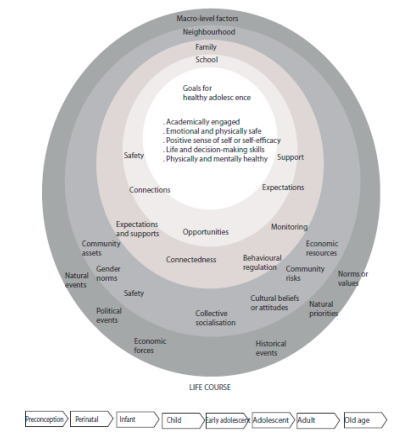
\includegraphics[width=2.08333in,height=\textheight]{images/Niveaus.png}

}

\caption{Verschillende niveau's van invloed}

\end{figure}
\end{frame}

\begin{frame}{3. De strategie}
\protect\hypertarget{de-strategie}{}
\end{frame}

\begin{frame}{Vijf fasen}
\protect\hypertarget{vijf-fasen}{}
\begin{itemize}
\tightlist
\item
  Fase 1: Mobilisatie inwoners van een bepaalde stad, gemeenschap of
  wijk en betrokkenen bij de opvoeding en ontwikkeling van de jeugd\\
\item
  Fase 2: Creëren van een gemeenschappelijke visie en taal, en het
  opzetten van een coherente planning structuur\\
\item
  Fase 3: Prioritering van de inspanningen obv onderzoek
  RF/BF-factoren\\
\item
  Fase 4: Lacunes en overlappingen programma's identificeren. Plan
  maken\\
\item
  Fase 5: Implementeren en evalueren
\end{itemize}

De kern van de aanpak is de analyse van de situatie en problemen binnen
een stad of wijk
\end{frame}

\begin{frame}{Vijf fasen in beeld}
\protect\hypertarget{vijf-fasen-in-beeld}{}
\begin{figure}

{\centering 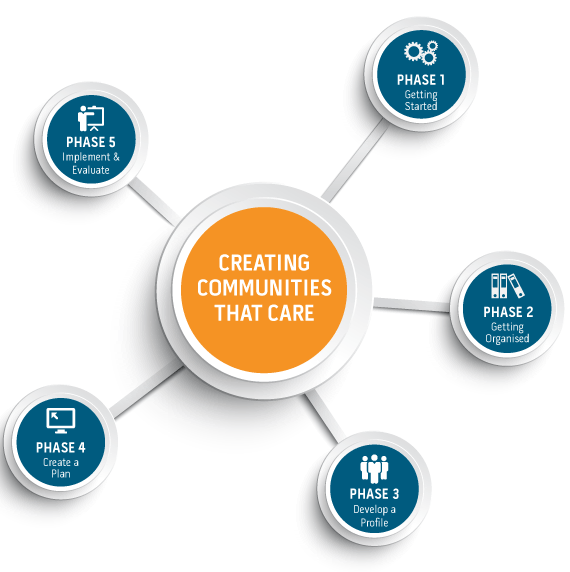
\includegraphics[width=2.08333in,height=\textheight]{images/Fasen.png}

}

\caption{Vijf fasen}

\end{figure}
\end{frame}

\begin{frame}{4. Vier kernelemementen}
\protect\hypertarget{vier-kernelemementen}{}
\begin{itemize}
\tightlist
\item
  Gebruik van zelfde implementatieproces\\
\item
  Het gebruik van epidemiologische data\\
\item
  Het gebruik van veelbelovende en effectieve programma's\\
\item
  Voortdurende evaluatie en herhalend onderzoek
\end{itemize}
\end{frame}

\begin{frame}{Hetzelfde implementatieproces}
\protect\hypertarget{hetzelfde-implementatieproces}{}
\begin{itemize}
\tightlist
\item
  Fase 1: Opstarten (Readiness meeting, introductietraining)\\
\item
  Fase 2: Geörganiseerd krijgen (Training Sleutelfiguren, Training
  Preventieteam)\\
\item
  Fase 3: Ontwikkelen profiel (Assessment training, Training
  programma's)\\
\item
  Fase 4: Plan maken (Planningstraining)\\
\item
  Fase 5: Implementatie en evaluatie (Training)
\end{itemize}
\end{frame}

\begin{frame}{Tijdlijn}
\protect\hypertarget{tijdlijn}{}
\begin{figure}

{\centering 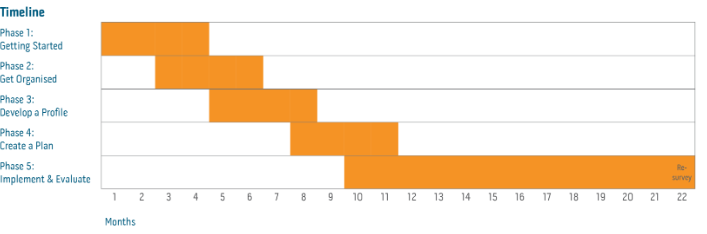
\includegraphics{images/Tijdlijn.png}

}

\caption{Fasen in tijd uitgezet}

\end{figure}
\end{frame}

\begin{frame}{Scholierenonderzoek}
\protect\hypertarget{scholierenonderzoek}{}
\begin{figure}

{\centering 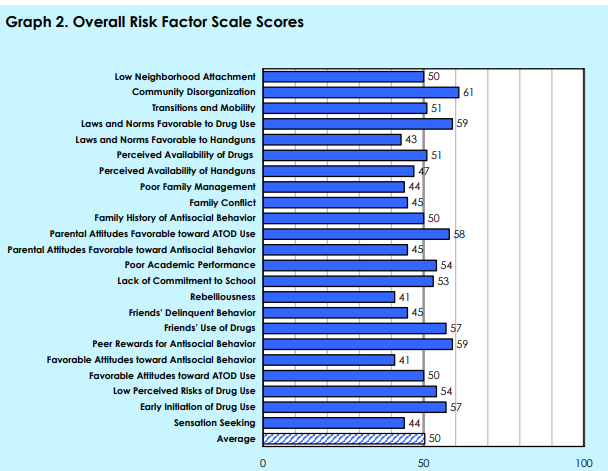
\includegraphics[width=2.08333in,height=\textheight]{images/Scholierenonderzoek.png}

}

\caption{Scholierenonderzoek}

\end{figure}

zie
\href{https://rothenbach-research.com/surveys/CTCYS_Sample_Report.pdf}{hier}
\end{frame}

\begin{frame}{Veelbelovend en effectief}
\protect\hypertarget{veelbelovend-en-effectief}{}
\begin{figure}

{\centering 
\includegraphics{images/Veelbelovend.png}

}

\caption{Veelbelovend en effectief}

\end{figure}
\end{frame}

\begin{frame}{5. CtC-Nederland experiment (1999-2004)}
\protect\hypertarget{ctc-nederland-experiment-1999-2004}{}
\end{frame}

\begin{frame}{Begin}
\protect\hypertarget{begin}{}
\begin{itemize}
\tightlist
\item
  Rapporten Junger-Tas (1996, 1997)\\
\item
  CtC als maatschappelijk antwoord op toenemende jeugdcriminaliteit en
  geweld
\item
  Gestructureerd, wijkgericht, effectief
\end{itemize}
\end{frame}

\begin{frame}{NIZW}
\protect\hypertarget{nizw}{}
\begin{itemize}
\tightlist
\item
  Uitzetten in vier gemeenten/wijken (Amsterdam, Rotterdam, Arnhem en
  Zwolle)\\
\item
  Trainingen ontwikkelen, implementeren en begeleiden
\item
  Scholierenonderzoek ontwikkelen en uitzettten
\item
  Veelbelovende en effectieve programma's
\end{itemize}
\end{frame}

\begin{frame}{Resultaten}
\protect\hypertarget{resultaten}{}
\begin{itemize}
\tightlist
\item
  Toename van de kwaliteit van planning en besluitvorming\\
\item
  Meer samenwerking tussen aanbieders\\
\item
  Meer coördinatie bij de programmering van preventieve maatregelen\\
\item
  Meer gerichtheid op onderliggende factoren (risico- en beschermende
  factoren)\\
\item
  Meer gebruik effectieve en veelbelovende benaderingen\\
\item
  Meer maatschappelijke betrokkenheid
\end{itemize}
\end{frame}

\begin{frame}{Algemene opmerking}
\protect\hypertarget{algemene-opmerking}{}
\begin{itemize}
\tightlist
\item
  Behoorde tot nieuwe generatie strategieën waarin onderzoek, effectieve
  programma's, implementatie en evaluatie worden samengebracht\\
\item
  Veel invloed van centrale overheid\\
\item
  Groeiende interesse
\end{itemize}
\end{frame}

\begin{frame}{6. CtC-Nederland interesse (2005-2015)}
\protect\hypertarget{ctc-nederland-interesse-2005-2015}{}
\begin{itemize}
\tightlist
\item
  Groeiende interesse waaronder Leeuwarden, Almere, provincie
  Zuid-Holland en diverse steden daar\\
\item
  Verdere kwaliteitsontwikkeling en controle
\item
  Ook internationale interesse (Nederlandse Antillen, Duitsland en
  Zweden)\\
\item
  Wetenschappelijke samenwerking met USA en Australie
\end{itemize}
\end{frame}

\begin{frame}{7. CtC-onderzoek (2008-2013)}
\protect\hypertarget{ctc-onderzoek-2008-2013}{}
\begin{figure}

{\centering 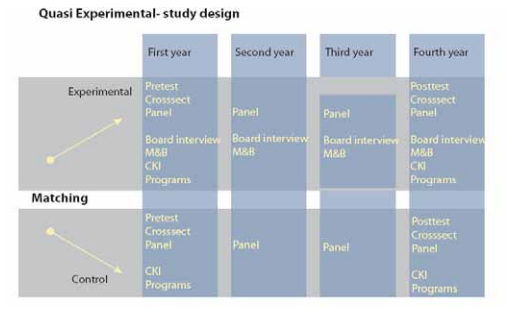
\includegraphics{images/Design.png}

}

\caption{Design}

\end{figure}
\end{frame}

\begin{frame}{Invloed op probleemgedragingen}
\protect\hypertarget{invloed-op-probleemgedragingen}{}
\begin{figure}

{\centering 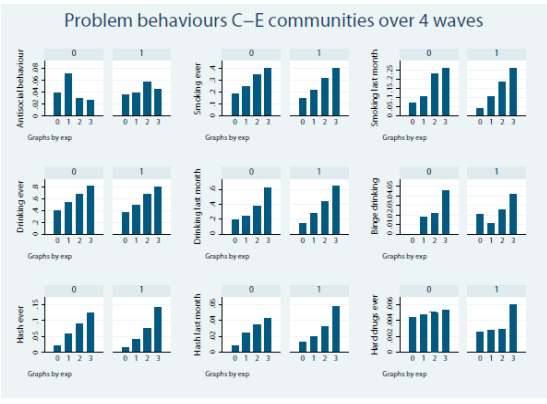
\includegraphics{images/PGInvloed.png}

}

\caption{Inlvoed op probleemgedragingen}

\end{figure}
\end{frame}

\begin{frame}{Onderliggende factoren}
\protect\hypertarget{onderliggende-factoren}{}
Ook op risicofactoren en beschermende factoren geen invloed
\end{frame}

\begin{frame}{Hoe dit te begrijpen?}
\protect\hypertarget{hoe-dit-te-begrijpen}{}
\begin{itemize}
\tightlist
\item
  Beperkte inzet van effectieve programma's\\
\item
  Geen invloed op inzet van deze programma's
\item
  Vertraagde en beperkte implementatie van CtC in de experimentele
  wijken\\
\item
  Gedeeltelijke contaminatie
\end{itemize}
\end{frame}

\begin{frame}{Procesonderzoek wel positief}
\protect\hypertarget{procesonderzoek-wel-positief}{}
CtC vooral een strategisch sturingsinstrument dat ertoe bijdraagt dat
instellingen uit de verschillende sectoren op het terrein van preventie
effectief en efficiënt samenwerken.

\begin{itemize}
\tightlist
\item
  CtC instrumenteert een nauwkeurige probleemanalyse\\
\item
  Het bevordert de samenwerking\\
\item
  Het geeft concreet richting aan een preventieve aanpak.
\end{itemize}
\end{frame}

\begin{frame}{8. Ontwikkelingen na 2015}
\protect\hypertarget{ontwikkelingen-na-2015}{}
Afname van de interesse voor CtC in Nederland - Minder geld\\
- Decentralisatie\\
- Geen centrale rol meer van één CtC partij\\
- Beperkte resultaten onderzoek
\end{frame}

\begin{frame}{9. Andere landen}
\protect\hypertarget{andere-landen}{}
\end{frame}

\begin{frame}{Amerika}
\protect\hypertarget{amerika}{}
\begin{quote}
CTC has shown to be effective in reducing alcohol use, substance use,
antisocial and violent behaviour, improving academic performance, and
strengthening protective factors. In addition to these improvements to
adolescent health and behaviour outcomes, large US trials of Communities
That Care have demonstrated that CTC communities are more likely to
adopt and implement evidence based programs compared to control
communities.
\end{quote}
\end{frame}

\begin{frame}{Amerikaanse publicaties}
\protect\hypertarget{amerikaanse-publicaties}{}
\href{https://www.communitiesthatcare.org.au/sites/default/files/youth_problem_behaviors_8_years_after_implementing_the_communities_that_care_prevention_system_-_a_community-randomized_trial.pdf}{Youth
problem behaviors 8 years after implementing the Communities That Care
prevention system: A community-randomized trial}

\href{https://www.communitiesthatcare.org.au/sites/default/files/variation_in_the_sustained_effects_of_the_communities_that_care_prevention_system_on_adolescent_smoking_delinquency_and_violence.pdf}{Variation
in the sustained effects of the Communities That Care prevention system
on adolescent smoking, delinquency, and violence}
\end{frame}

\begin{frame}{Australië}
\protect\hypertarget{australiuxeb}{}
\begin{quote}
Research around adolescent alcohol use in the Australian context has
shown that community-family-school coalitions can reduce youth alcohol
use. Alcohol and drug policies at the school and community levels can
also make a potentially important contribution to reducing community
rates of alcohol and drug use. In particular, there is evidence that
community policies for the sale and supply of alcohol effect early
adolescent alcohol use.
\end{quote}
\end{frame}

\begin{frame}{Australische publicaties}
\protect\hypertarget{australische-publicaties}{}
\href{https://www.communitiesthatcare.org.au/sites/default/files/ctc_prospectus2022.pdf}{CtC-Prospectus}

\href{https://www.communitiesthatcare.org.au/sites/default/files/toumbourou_et_al_2018.pdf}{Student
survey trends in reported alcohol use and influencing factors in
Australia}

\href{https://www.communitiesthatcare.org.au/sites/default/files/longitudinal_effects_of_school_drug_policies_on_student_marijuana_use_in_washington_state_and_victoria_australia.pdf}{Longitudinal
effects of school drug policies on student marijuana use in Washington
State, US and Victoria, Australia}
\end{frame}

\begin{frame}{Duitsland}
\protect\hypertarget{duitsland}{}
\begin{itemize}
\tightlist
\item
  Ook in Duitsland actief sinds 2010\\
\item
  Op groot aantal plekken uitgezet
\item
  Ook groot onderzoek\\
\item
  \href{https://www.ctc-info.de/nano.cms/umsetzung}{Hier} vind je
  informatie, maar niet erg up to date.
\end{itemize}
\end{frame}

\begin{frame}{Europa}
\protect\hypertarget{europa}{}
\begin{figure}

{\centering 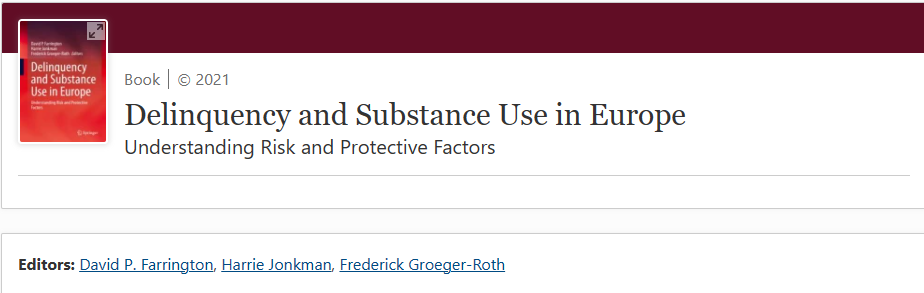
\includegraphics{images/Springer.png}

}

\caption{Delinquncy and Substance Use in Europe}

\end{figure}
\end{frame}

\begin{frame}{Europa 2}
\protect\hypertarget{europa-2}{}
Onderzoek van Communities that Care in Europa (Engeland, Nederland,
Duitsland, Kroatië en Cyprus)

\begin{itemize}
\tightlist
\item
  Vergelijking prevalentie van delinquentie en alcohol en drugsgebruik
  in deze landen\\
\item
  prevalentie van belangrijke risico en beschermende factoren in deze
  landen\\
\item
  onderzoek naar de relatie tussen problemen en onderliggende factoren.
\end{itemize}
\end{frame}

\begin{frame}{11. Discussie}
\protect\hypertarget{discussie}{}
\end{frame}

\begin{frame}{Betekenis voor sociale politiek}
\protect\hypertarget{betekenis-voor-sociale-politiek}{}
\begin{itemize}
\tightlist
\item
  Promotie van welzijn, preventie van probleemgedrag, samenhangende
  sociale determinanten moet een van de kern zijn van jeugdpolitiek op
  internationaal, nationaal en lokaal niveau
\item
  Gemeenschappen (steden en wijken) hebben onderzoekssystemen nodig om
  incidentie en prevalentie van jeugdproblemen te kunnen onderzoeken en
  de ontwikkelingen ervan bij te horen
\item
  Samenwerken wordt al lang over gesproken, ook op het terrein van
  sociale politiek. Hoe je dat voor elkaar kunt krijgen is onduidelijk.
  Dit is een goed voorbeeld
\item
  Over effectieve programma's kun je lang praten. Onderzoekers, politici
  en praktijkmensen hebben een manier nodig om dit op bredere schaal uit
  te zetten. CtC is een voorbeeld hiervan
\end{itemize}
\end{frame}

\begin{frame}{Betekenis vanuit onderzoek}
\protect\hypertarget{betekenis-vanuit-onderzoek}{}
\begin{itemize}
\tightlist
\item
  Hoe kunnen we lokale onderzoeksgegevens gebruiken?
\item
  Hoe kunnen wetenschap, politiek en praktijk samenwerken?
\item
  Preventie moet weten hoe zaken moeten worden versterkt en voorkomen.
  RF en BF inzichten is het beste wat we hebben. Wel meer in samenhang
  bekijken en ook de verschillende niveaus bekijken
\item
  Nog steeds weten we weinig van de invloed van sociaal investeren en
  onderzoek op dit terrein blijft nodig
\end{itemize}
\end{frame}

\begin{frame}{CtC-Bezoek}
\protect\hypertarget{ctc-bezoek}{}
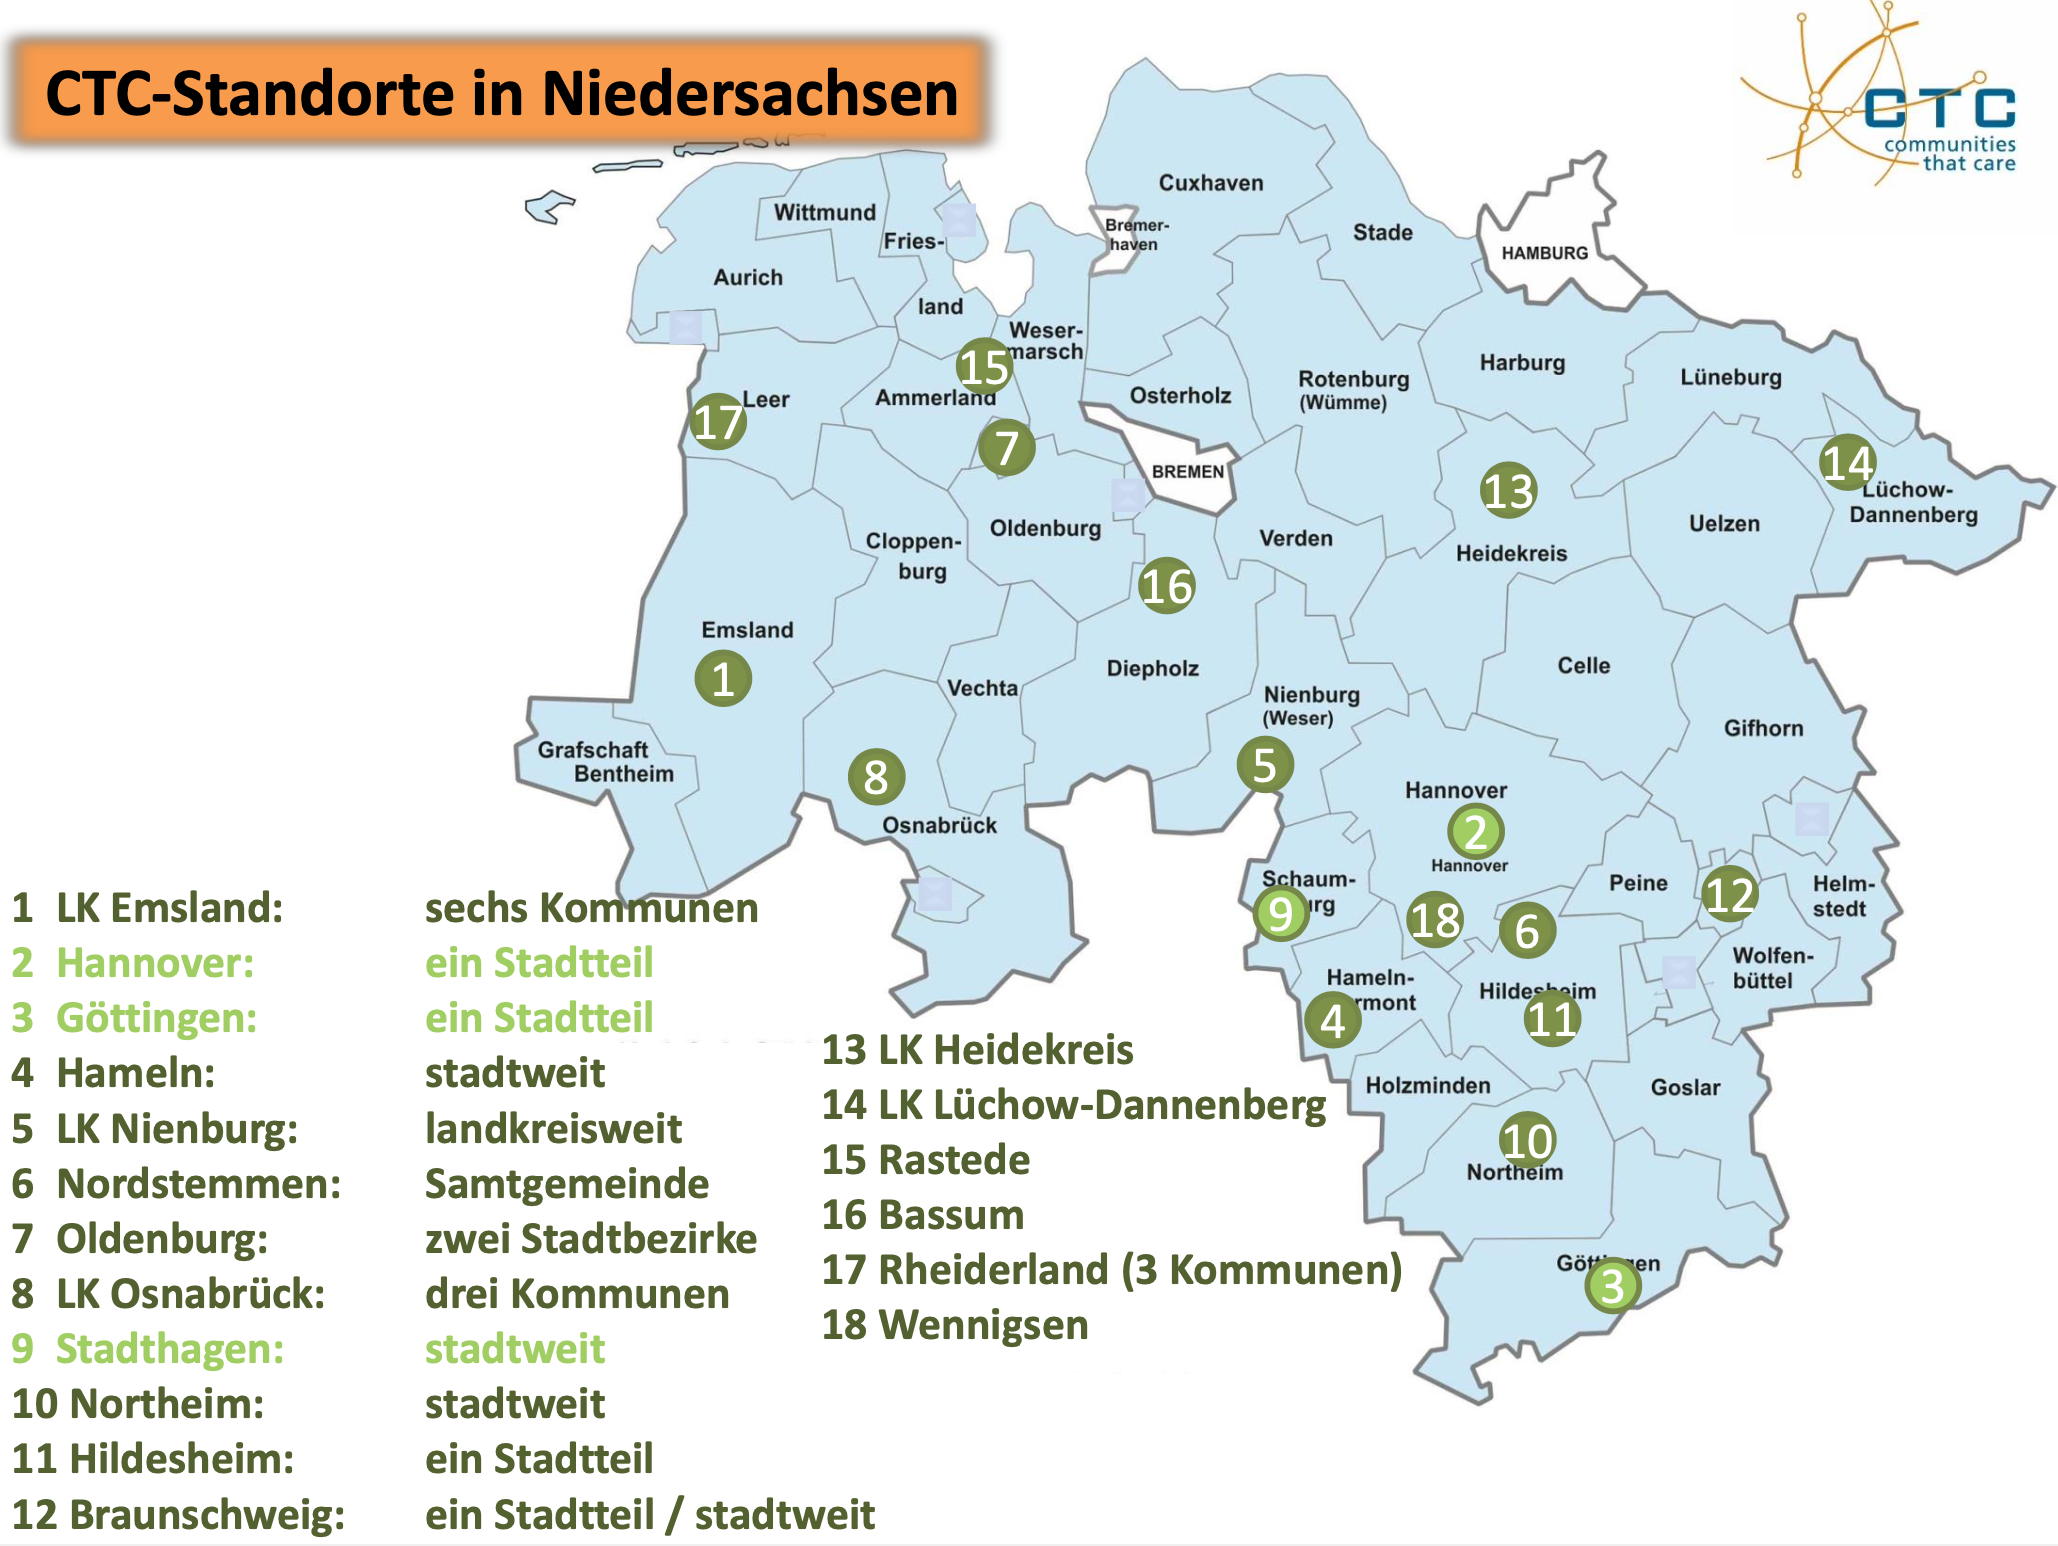
\includegraphics{images/CTCDL.png} \#\# Tot slot

Hartelijke dank

dr. Harrie Jonkman

Zuideinde 387e 1035PE Amsterdam

harriejonkman@xs4all.nl

www.harriejonkman.nl
\end{frame}



\end{document}
